\documentclass[a4paper, 12pt, oneside]{book}
\usepackage[left=2.5cm,right=2.5cm,top=2.5cm,bottom=2.5cm]{geometry}
\usepackage[spanish, es-noshorthands,activeacute]{babel} % es-noshorthands es para que no tenga problemas con tikz
\usepackage[latin1]{inputenc}
\usepackage{graphicx}
\usepackage{amssymb}
\usepackage{amsthm}
\usepackage{amsmath}
\usepackage{makeidx}
\usepackage{color}
\usepackage{algpseudocode}

\hyphenation{Polyno-mialtime}
%%%%%%%%%%%%%%%%%%%%%%%%%%%%%%%%%%%%%%%%%%%%%%%%%%%%%%%%%%%%%%%%%%%%
\newtheorem{definicion}{Definici\'on}[chapter]
\newtheorem{lema}{Lema}[chapter]
\newtheorem{proposicion}{Proposici\'on}[chapter]
\newtheorem{teorema}{Teorema}[chapter]
\newtheorem{corolario}{Corolario}[chapter]
\newtheorem{observacion}{Observaci\'on}[chapter]
\newtheorem{ejemplo}{Ejemplo}[chapter]
\newtheorem{ejercicio}{Ejercicio}[chapter]
%añadir [chapter] al final de cada comando si se desea que la numeración vaya acorde al capítulo

%%%%%%%%%%%%%%%%%%%%%%%%%%%%%%%%%%%%%%%%%%%%%%%%%%%%%%%%%%%%%%%%%%%%%
\renewcommand{\thesection}{\arabic{section}}
%%%%%%%%%%%%%%%%%%%%%%%%%%%%%%%%%%%%%%%%%%%%%%%%%%%%%%%%%%%%%%%%%%%%%




\begin{document}
	\pagenumbering{roman}
	%-------------------------------------------------------------------------Inicio P\'{a}gina del T\'{\i}tulo
	\begin{titlepage}
		
		
\includegraphics[scale=0.18]{logo-facultad-ciencias-uma}
		
		\vskip2truecm
		
		\begin{center}
			
			% Upper part of the page. The '~' is needed because \\
			% only works if a paragraph has started.
			
			%\includegraphics[width=0.35\textwidth]{\textbf{logo-facultad-ciencias-uma}}~\\[1cm]
			
			
			%\textsc{\LARGE Universidad de M\'{a}laga}
			
			%\textsc{Facultad de ciencias}\\ [1.5cm]
			
			%\textsc{\Large Trabajo Fin de Grado}\\[0.5cm]
			
			% Title
			%\noindent\rule{\textwidth}{0.4mm}
			{ \huge \bfseries T\'{\i}tulo del tfg en espa\~{n}ol  \\[0.4cm] }
			
			%\noindent\rule{\textwidth}{0.4mm}
			\vskip1truecm
			
			{ \huge \bfseries T\'{\i}tulo del tfg en ingl\'es \\[0.4cm] }
			
			%\noindent\rule{\textwidth}{0.4mm}
			
			
			\vskip1truecm
			
			{\Large Trabajo Fin de Grado en Matem\'aticas} \\
			
			{\Large Universidad de M\'alaga} \\
			
			%\vfill
		\end{center}
		
		\vskip2truecm
		
		\noindent\rule{\textwidth}{0.4mm}
		
		\vskip.2truecm
		
		
		{\bf Autor:} {Rafael Requena Garrido}\\
		
		{\bf \'{A}rea de conocimiento y/o departamento:} \\
		
		{\bf Fecha de presentaci\'{o}n: (mes y a\~{n}o)}\\
		
		{\bf Tema:}\\
		
		{\bf Tipo:} {(trabajo de revisi\'on bibliogr\'afica, de iniciaci\'on a la investigaci\'on,...)}\\
		
		{\bf Modalidad:} {(individual o grupal)}\\
		
		{\bf N\'umero de p\'aginas (sin incluir introducci\'on, bibliograf\'{\i}a ni anexos):}\\
		
		
		
		
	\end{titlepage}
	%-------------------------------------------------------------------------Fin P\'{a}gina del T\'{\i}tulo
	%----------------P\'agina en blanco--------------------------------------------------------------
	\newpage
	\mbox{}
	\thispagestyle{empty}
	%----------------Fin p\'agina en blanco---------------------------------------------------
	\begin{titlepage}
		\begin{center}
			
			
			
			\textsc{\Large DECLARACI\'{O}N DE ORIGINALIDAD DEL TFG}\\[0.5cm]
			\bigskip
			
			%\noindent\rule{\textwidth}{0.4mm}
			\vskip2truecm
			% Author and tutor
			%\begin{minipage}{0.4\textwidth}
			%\begin{flushleft} \large
			%\emph{Autor:}\\
			%\textsc{Nombre y Apellidos del autor}
			%\end{flushleft}
			%\end{minipage}
		\end{center}
		
		D./D\~{n}a. \textit{(nombre del autor)}, con DNI (NIE o pasaporte) \textit{(DNI, NIE o pasaporte)}, estudiante del Grado en \textit{(titulaci\'{o}n)} de la Facultad de Ciencias de la Universidad de M\'{a}laga,\\
		\textbf{DECLARO:}\\
		
		Que he realizado el Trabajo Fin de Grado titulado ``\textit{(T\'{i}tulo)}'' y que lo presento para su evaluaci\'{o}n. Dicho trabajo es original y todas las fuentes bibliogr\'{a}ficas utilizadas para su realizaci\'{o}n han sido debidamente citadas en el mismo.\\
		\medskip
		
		De no cumplir con este compromiso, soy consciente de que, de acuerdo con la normativa reguladora de los procesos de evaluaci\'on de los aprendizajes del estudiantado de la Universidad de M\'alaga de 23 de julio de 2019, esto podr\'a conllevar la calificaci\'on de suspenso en la asignatura, sin perjuicio de las responsabilidades disciplinarias en las que pudiera incurrir en caso de plagio.
		\bigskip
		
		
		Para que as\'{i} conste, firmo la presente en M\'{a}laga, el \textit{(fecha)}\\
		
		
		
		%\vfill
		
		%\noindent\emph{Tutor y co-tutor (si lo hubiera):} \\
		%{\bf Prof. Dr. Nombre y apellidos del tutor}
		%\bigskip
		%\bigskip
		%\bigskip
		
		%\noindent \emph{Palabras Clave:}\\
		%\textsc{poner aqu\'{\i} las palabras clave.}
		
		\vskip.3truecm
		% Bottom of the page
		
		\qquad\qquad\qquad {Fdo:..............................................................}
		
	\end{titlepage}
	
	
	
	
	
	
	
	
	
	
	
	\tableofcontents
	
	\addcontentsline{toc}{chapter}{Resumen} 
	\addcontentsline{toc}{chapter}{Abstract} 
	\addcontentsline{toc}{chapter}{Introducci\'on}
	
	\pagebreak
	
	{\let\clearpage\relax
		
		{\Large \textbf{El T\'{\i}tulo aqu\'{\i}}}\\
		
		\chapter*{Resumen}
	}
	Texto.
	
	\vfill
	
	\textbf{Palabras clave:}\\
	
	\textsc{poner aqu\'{\i} las palabras clave.}
	
	\pagebreak
	
	{\let\clearpage\relax
		
		{\Large \textbf{El T\'{\i}tulo (en ingl\'{e}s) aqu\'{\i}}}\\
		
		\chapter*{Abstract}
	}
	
	Text. 
	
	\vfill
	
	\textbf{key words:}\\
	
	\textsc{key words.}
	
	\chapter*{Introducci\'on}
	
	
	\chapter{Optimizaci\'{\o}n combinatoria}
	\pagenumbering{arabic}
	\setcounter{page}{1}
	
	\section{Conceptos generales}
	Para comprender con mayor claridad el objetivo de la optimizaci\'{o}n y los elementos que juegan un papel clave en la misma, procederemos a introducirla mediante un ejemplo:
	\\
	
	Supongamos que una compa\~{n}\'ia fabrica y vende dos modelos de mesas, $M_{1}$ y $M_{2}$ . Para su fabricaci\'on, es necesario un trabajo manual de 20 y 30 minutos para los modelos $M_{1}$ y $M_{2}$, respectivamente, m\'as un trabajo de m\'aquina de 20 minutos para el modelo $M_{1}$  y de 10 minutos para el modelo $M_{2}$. Para el trabajo manual se dispone de 100 horas al mes, mientras que, para el de m\'aquina, 80 horas. Sabiendo que el beneficio por unidad es de 150 y 100 euros para $M_{1}$ y $M_{2}$, respectivamente, queremos planificar la producci\'on de manera que obtengamos el beneficio m\'aximo.
	\\
	
	Si llamamos $x$ = n\'umero de mesas $M_{1}$ e $y$ = n\'umero de mesas de $M_{2}$, podemos definir la funci\'on beneficio $f(x,y) = 150x + 100y$. Por otro lado, pasando el tiempo a horas, las condiciones dadas en el enunciado se traducen a:
	
	$$\frac{1}{3}x + \frac{1}{2}y \leq 100$$
	$$\frac{1}{3}x + \frac{1}{6}y \leq 80$$
	
	Si juntamos todo para escribirlo como es habitual en los textos de optimizaci\'on, tenemos que nuestro problema se modela como sigue:
	
	$$f(x,y) = 150x + 100y$$
	$$s.a\ \frac{1}{3}x + \frac{1}{2}y \leq 100$$
	$$\frac{1}{3}x + \frac{1}{6}y \leq 80$$
	$$x\geq 0, y\geq 0, x,y \in \mathbb{Z} $$
	
	De este modo, nuestro problema se reduce a encontrar un par $(x,y)$ que mamximice a la funci\'on $f$ y verifique las restricciones anteriores.
	\\
	
	Formalmente, un problema de optimizaci\'on se puede describir (\textbf{citar tesis Pepe}) como una tupla $(D, X, f, R)$ dinde:
	
	\begin{enumerate}
		\item $D = \{D_{1},...,D_{n}\}$ es un conjunto de dominios.
		\item $X = \{x_{1},...,x_{n}\}$ es un conjunto de variables tal que para cada $i\in \{1,...,n\}, x_{i} \in D_{i}$.
		\item $f : D_{1} \times ... \times D_{n} \longrightarrow \mathbb{R^{+}}$ se denomina \textit{funci\'on objetivo}, para la cual estaremos interesados en conocer sus m\'aximos o m\'inimos.
		\item \textit{R} es un conjunto de restricciones sobre las variables.
	\end{enumerate}
	
	Por otro lado, definimos el conjunto $S\subseteq D_{1} \times ... \times D_{n}$ en el que se verifican las restricciones de \textit{R} como el \textit{espacio de b\'usqueda} del problema y, a cada $s\in S$, una \textit{soluci\'on posible (o factible)} del problema. As\'i, una soluci\'on del problema es un elemento $s^{*}\in S$ tal que $f(s^{*}) \geq f(s), \forall s \in S$. A $s^{*}$ se le denomina \textit{\'optimo global} del problema. Usualmente se sigue la nomenclatura anterior para los problemas de optimizaci\'on en los que maximizamos la funci\'on $f$, mientras que cuando lo que buscamos es minimizarla, nos referimos a ella como \textit{funci\'on de costos}.
	\\
	
	Existen diversas formas de clasificar a los problemas de optimizaci\'on. Como no existe un m\'etodo \'unico para resolver todos los problemas posibles, es importante analizar en qu\'e categor\'ia entra el problema en cuesti\'on ya que, de esta manera, podremos emplear algoritmos que se ajusten mejor al mismo, ya sea reduciendo el tiempo de c\'alculo y/o hallando soluciones m\'as aproximadas o exactas, por ejemplo.
	\\
	
	As\'i, podemos realizar una primera clasificaci\'on atendiendo a la continuidad o no de las variables. En el caso m\'as general, diremos que estamos frente a un problema de \textit{Optimizaci\'on Continua} cuando todas las variables del problema sean de tipo continuo. Dentro de este tipo de problemas, cobran especial importancia los problemas de \textit{Optimizaci\'on Conveza}, en los cuales tenemos que minimizar (en general) una \textit{funci\'on convexa} (usalmente llamada \textit{funci\'on de costos}) sujeta a un conjunto soluci\'on convexo. Cuando la funci\'on objetivo y las restricciones son lineales, decimos que estamos frente a un problema de \textit{Optimizaci\'on Convexa Lineal} o \textit{Programaci\'on Lineal}, mientras que cuando no lo son, decimos que el problema es de \textit{Programaci\'on no Lineal.}
	\\
	
	En cambio, si las variables son de tipo discreto, es decir, solo pueden tomar valores enteros, decimos que el problema es de \textit{Optimizaci\'on Combinatoria}. Finalmente, decimos que un problema es de \textit{Optimizaci\'on Mixta} cuando tiene algunas variables de tipo continuo y otras de tipo discreto.
	\\
	
	En cuanto a los distintos m\'etodos de resoluci\'on de problemas de optimizaci\'on, aqu\'i tambi\'en encontramos difersas formas de clasificarlos:
	
	\begin{itemize}
		\item Resoluci\'on mediante c\'alculo,
		\item Resoluci\'on mediante t\'ecnicas de b\'usquedas.
		\item Resoluci\'on mediante t\'ecnicas de convergencia de soluciones
	\end{itemize}
	
	Los m\'etodos de resoluci\'on por c\'alculo hacen uso del c\'alculo de derivadas para determinar qu\'e valores del dominio de la funci\'on presentan m\'aximos y m\'inimos. Son m\'etodos muy potentes, pero requieren mucha capacidad de c\'omputo y que la funci\'on objetivo y las restricciones cumplan una serie de condiciones (condiciones de continuidad, derivabilidad, etc.). En la pr\'actica estos m\'etodos no suelen utilizarse, ya que los problemas no suelen cumplir las condiciones necesarias para la aplicaci\'on de estos m\'etodos y tienen demasiada variables como para que sean eficientes. Un ejemplo cl\'asico de estos m\'etodos, es el m\'etodo de los multiplicadores de Lagrange.
	\\
	
	En los m\'etodos de resoluci\'on mediante t\'ecnicas de b\'usquedas, podemos encontrar desde m\'etodos exactos como el tradicional algoritmo del s\'implex (para problemas de Programaci\'on Lineal) y sus variantes hasta t\'ecnicas metaheur\'isticas como la \textit{b\'usqueda tab\'u} o el \textit{recocido simulado (simulated annealing)}, tambi\'en conocido como algoritmo de cristalizaci\'on simulada.
	\\
	
	Por otro lado, la mayor\'ia de t\'ecnicas de convergencia de soluciones son de tiempo metaheur\'istico. Se basan en generar gran cantidad de soluciones, determinar cu\'ales son las mejores y, a partir de ellas, generar otro conjunto de soluciones a analizar, repitiendo el proceso hasta que estas soluciones que vamos generando converjan a una. Por lo tanto, dentro de este grupo podemos encontrar t\'ecnicas de tipo iterativo, como el cl\'asico m\'etodo de Newton o el m\'etodo de descenso del gradiente hasta los \textit{algoritmos gen\'eticos} (de tipo metaheur\'istico), que se enmarcan dentro de los \textit(algoritmos evolutivos), diendo estos dos \'ultimos muy empleados en el \'are de la inteligencia artificial.
	\\
	
	Hecho este breve contexto, estamos en disposici\'on de centrarnos en el caso que nos ata\~{n}e. La optmizaci\'on combinatoria es una rama de la optimizaci\'on relacionada con la investigaci\'on operativa, la teor\'ia algor\'itmica y la teor\'ia de la complejidad computacional (\textbf{citar wiki/art\'iculo jgarcia}). Observemos que, para un problema de optimizaci\'on combinatoria $P = (D, X, f, R)$, el conjunto $S\subseteq D$ de las posibles soluciones de $P$ es finito, lo cual nos lleva a encontrar un m\'etodo simple con el que hallar el \'optimo global de $P$, que consiste en examinar todas las posibles soluciones del problema. Sin embargo, en la pr\'actica, en la mayor\'ia de problemas de optimizaci\'on combinatoria no es posible la aplicaci\'on de este m\'etodo debido a que el espacio de b\'usqueda crece exponencialmente con el tama\~{n}o del problema (o tama\~{n}o de la instancia del problema), lo cual hace que el coste computacional y el tiempo necesario para examinar cada una de las posibles soluciones sea inviable.
	\\
	
	El \textit{tama\~{n}o de una instancia} (\textbf{citar Brassard}) se corresponde formalmente al n\'umero de bits necesarios para representar la instancia en un ordenador, utilizando alg\'un esquema de codificaci\'on definido con precisi\'on y razonablemente compacto. No obstante, para que los an\'alisis sean m\'as claros, normalmente emplearemos la palabra "tama\~{n}o" para referirnos a cualquier n\'umero entero que mida de alg\'un modo el n\'umero de componentes de una instancia. Por ejemplo, cuando hablamos de ordenar, usualmente medimos el tama\~{n}o de la instancia por el n\'umero de elementos a ordenar, independientemente de que dichos elementos necesiten m\'as de un bit para ser representados en un ordenador.
	\\
	
	Esta necesidad de resolver instancias de problemas cada vez m\'as grandes con un coste computacional aceptable nos lleva a desarrollar algoritmos que, aunque no nos proporcionan soluciones exactas, si nos permiten obtener soluciones aproxiamadas razonablemente buenas. Son los ya mencionados algoritmos heur\'isticos.
	
	\section{Complejidad. Problemas P vs NP}
	
	Uno de los objetivos de este documento es analizar la eficiencia de una serie de algoritmos en la resoluci\'on de un problema de optimizaci\'on combinatoria. Para ello, resulta necesario la introducci\'on de unos cuantos conceptos con los que analizarlos.
	\\
	
	La teor\'ia de la complejidad computacional (o teor\'ia de la complejidad inform\'atica) es una rama de la teor\'ia de la computaci\'on que trata de clasificar los problemas computacionales en base a si pueden ser o no resueltos con una cantidad determinada de tiempo y memoria, lo que suele denominarse como su \textit{dificultad inherente}.
	\\
	
	A continuaci\'on presentamos la notaci\'on $O$ grande, tambi\'en conocida como notaci\'on de \textit{Landau}, usada frecuentemente para clasificar funciones en base a su velocidad de crecimiento, es decir, su orden de magnitud. Dado que se basa en su comportamiento en casos l\'imite, define lo que se denomina \textit{coste as\'intotico} de los algoritmos.
	\\
	
	Sean dos funciones $f,g: \mathbb{R} \longrightarrow \mathbb{R}$. Decimos que $f(n)$ es $O(g(n))$ (o que $f(n) = O(g(n))$) si y solo si existen $n_{0},c > 0$ tales que $|f(n)| \leq c|g(n)|$ para todo $n > n_{0}$.
	\\
	
	La notaci\'on $O(f)$ tiene las siguientes propiedades (\textbf{citar webdiis.unizar}), cualesquiera que sean las funciones $f,g$ y $h$:
	
	\begin{enumerate}
		\item Para todo $c \in \mathbb{R^{+}}$, $$ f(n) = O(g(n)) \Longleftrightarrow c \cdot f(n) = O(g(n)) $$
		
		\item Si $f(n) = O(g(n))$ y $g(n) = O(h(n))$ entonces $f(n) = O(h(n))$.
		
		\item $O(f+g) = O(max(f,g))$. Se demuestra f\'acilmente haciendo uso de las desigualdades
		
		\[\left .\begin{array}{ll}
			f \leq max(f,g) \\
			g \leq max(f,g)
		\end{array}\right\}\rightarrow f + g \leq max(f,g) + max(f,g) \leq 2\, max(f,g)
		\]
		
		Frecuentemente esta propiedad se aplica as\'i: si $f_{1} = O(g_{1})$ y $f_{2} = O(g_{2})$, entonces $f_{1} + f_{2} = O(max(g_{1},g_{2}))$.
		
		\item Si $f_{1} = O(g_{1})$ y $f_{2} = O(g_{2})$, entonces $f_{1} \cdot f_{2} = O(g_{1} \cdot g_{2})$.
		
		\item Para todo $c \in \mathbb{R^{+}}$, 
		$$f = O(g) \Longleftrightarrow c + f = O(g)$$
		
		Es consecuencia inmediata de la regla de la suma.
		
	\end{enumerate}
	
	De este modo, tenemos la siguiente jerarqu\'ia para las formas de crecimiento asint\'otico m\'as importantes:
	
	$$ O(1) \subset O(log\,n) \subset O(n) \subset O(n\,log\,n) \subset O(n^{2}) \subset O(n^{3}) \subset O(2^{n}) $$
	
	\begin{figure}[h]
		\centering
		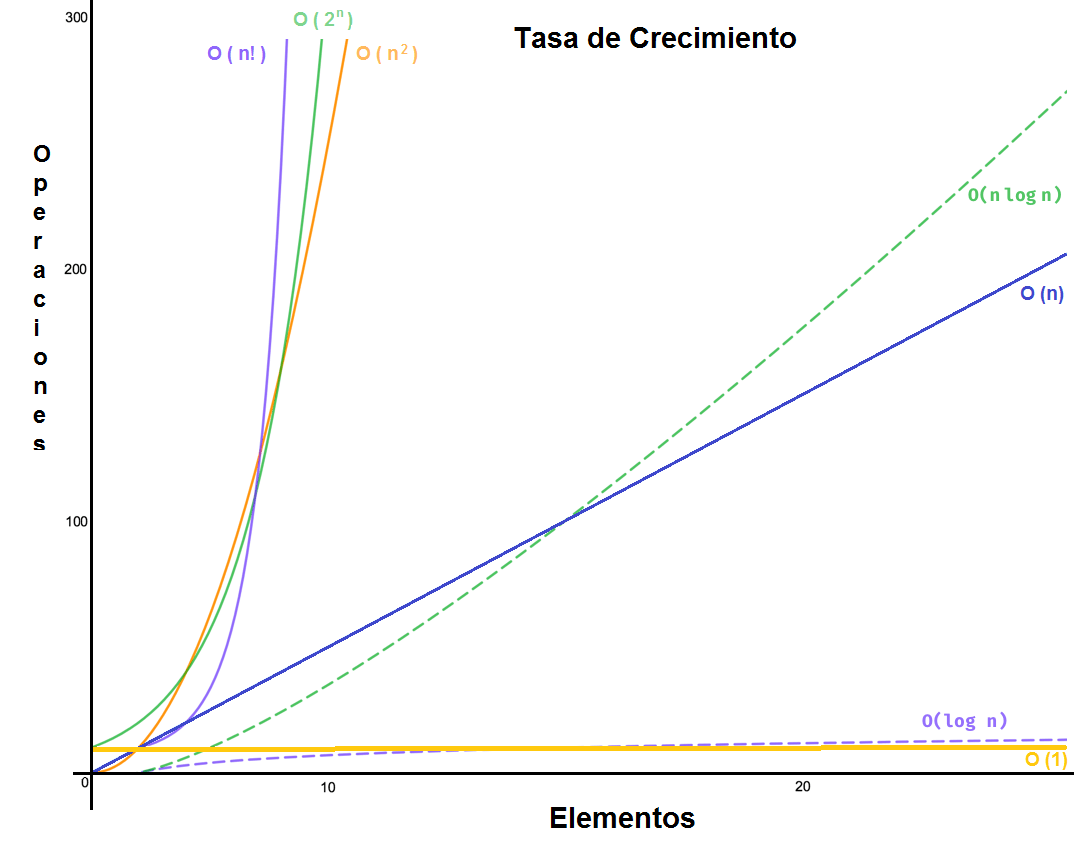
\includegraphics[scale = 0.4]{grafico-complejidad-computacionala3.png}
		\caption{Formas de crecimiento asint\'otico m\'as importantes}
		\label{fig:complejidad}
	\end{figure}
	
	\textbf{?`Comentar aqu\'i algo acerca de que hay que tener cuidado a la hora de comparar algoritmos en base a su coste asint\'otico? Por ejemplo con los algoritmos de Karatsuba, Toom-Cook y Sch\"onhage-Strassen para el producto.}
	\\
	
	Sin embargo, ?`qu\'e significa que un algoritmo sea eficiente? ?`Significa que toma un tiempo en $O(n\,log\,n)$? ?`$O(n^{2})$? Depender\'a del problema a resolver.
	\\
	
	Decimos que un algoritmo es eficiente (\textbf{citar Brassard}) si existe un polinomio $p(n)$ tal que el algoritmo puede resolver cualquier instancia del problema de tama\~{n}o \textit{n} en un tiempo $O(p(n))$. Se dice entonces que el algoritmo es de \textit{tiempo polin\'omico} y que los problemas que se resuelven con dicho algoritmo son resolubles en tiempo polin\'omico. Sin embargo, cuando el tiempo de ejecuci\'on de un algoritmo no se puede expresar mediante una f\'ormula polin\'omica, se dice que dicho algoritmo y su problema asociado son de \textit{tiempo exponencial}. Cuando un problema solo se puede resolver mediante algoritmos de tiempos exponenciales, se dice que el problema es \textit{intratable}.
	\\
	
	Para el prop\'osito de este trabajo, nos centraremos en el caso de los problemas de decisi\'on, que son aquellos problemas que tienen como respuesta s\'i o no, o equivalentemente, verdadero o falso. Un problema de decisi\'on puede considerarse como la definici\'on de un conjunto de instancias en los que la respuesta correcta es s\'i.
	\\
	
	Todas estas consideraciones anteriores nos sirven de base para la introducci\'on de los siguientes conceptos:
	
	\begin{definicion}
		Una clase de complejidad es un conjunto de problemas que poseen la misma complejidad computacional (\textbf{citar wiki)}.
	\end{definicion}
	
	\begin{definicion}
		La clase de problemas de decisi\'on que pueden ser resueltos por una m\'aquina de Turing determinista en un tiempo polinomial es conocida como clase P (Poly\-nomial-time)
	\end{definicion}
	
	En t\'erminos generales, P corresponde a la clase de problemas que, de forma realista, se pueden \textbf{resolver} con un ordenador. La mayor\'ia de problemas habituales (ordenaci\'on, b\'usqueda, etc.) pertenecen a esta clase.
	
	\begin{definicion}
		Llamamos clase NP (Non-Deterministic Polynomial-time) a aquella formada por los problemas de decisi\'on que son \textbf{verificables} por m\'aquinas de Turing no determinista en tiempos polin\'omicos.
	\end{definicion}
	
	Una relaci\'on evidente entre ambas clases es que $P \subset NP$, ya que si podemos resolver un problema en tiempo polin\'omico, evidentemente tambi\'en podemos verificarlo en tiempo polin\'omico.
	\\
	
	Otro importante subconjunto de la clase \textit{NP} son los problemas \textit{NP-completo}.(\textbf{citar wiki a continuaci\'on})
	
	\begin{definicion}
		Un problema de decisi\'on C es NP-completo si:
		\begin{enumerate}
			\item C $\in$ NP
			\item Todo problema de NP es \textbf{reducible polinomialmente} a C en tiempo polin\'omico.
		\end{enumerate}
	\end{definicion}
	
	Una reducci\'on polin\'omica de \textit{L} en \textit{C} es un algoritmo de tiempo polin\'omico que transforma instancias de \textit{L} en instancias de \textit{C}, de manera que la respuesta a \textit{C} es positiva si y solo si lo es la de \textit{L}. De forma general, la clase \textit{NP-completo} corresponde a la de los problemas que pueden verificarse de forma sencilla pero que solo pueden resolverse por fuerza bruta. Algunos de los problemas que pertenecen a esta clase son el \textbf{problema de satisfacibilidad booleana} (SAT), el \textbf{problema de la mochila} (com\'unmente abreviado por KP), el \textbf{problema del ciclo hamiltoniano} o el \textbf{problema del viajante}. Esta clase tiene la propiedad (\textbf{citar wiki)} de que si alg\'un problema \textit{NP-completo} puede ser resuelto en tiempo polin\'omico, entonces todo problema en \textit{NP} tiene una soluci\'on en tiempo polin\'omico, es decir, $P = NP$.
	\\
	
	A pesar de a\~{n}os de investigaci\'on, la cuesti\'on de si $P = NP$ contin\'ua a\'un abieta y es considerado uno de los problemas del milenio. La importancia de este resultado radica en el hecho de que si $P \neq NP$, entonces los problemas \textit{NP-completo} son intratables, ya que si alg\'un problema en \textit{NP} requiere m\'as tiempo que uno polinomial, entonces uno \textit{NP-completo} tambi\'en.
	\\
	
	Una clase m\'as general de problemas no restringida a los problemas de decisi\'on es la clase de complejidad \textit{NP-dif\'icil} (\textit{NP-hard}). (\textbf{citar wiki para la def.})
	
	\begin{definicion}
		La clase de complejidad NP-dif\'icil es el conjunto que contiene a los problemas C tales que todo problema L en NP puede ser transformado polinomialmente en C.
	\end{definicion}
	
	Esta clase contiene a aquellos problemas que son, como m\'inimo, tan dif\'iciles como un problema de \textit{NP}. De esta forma, la clase \textit{NP-completo} puede definirse como la intersecci\'on entre las clases \textit{NP} y \textit{NP-dif\'icil}. (\textbf{imagen de wiki})
	
	\begin{figure}[h]
		\centering
		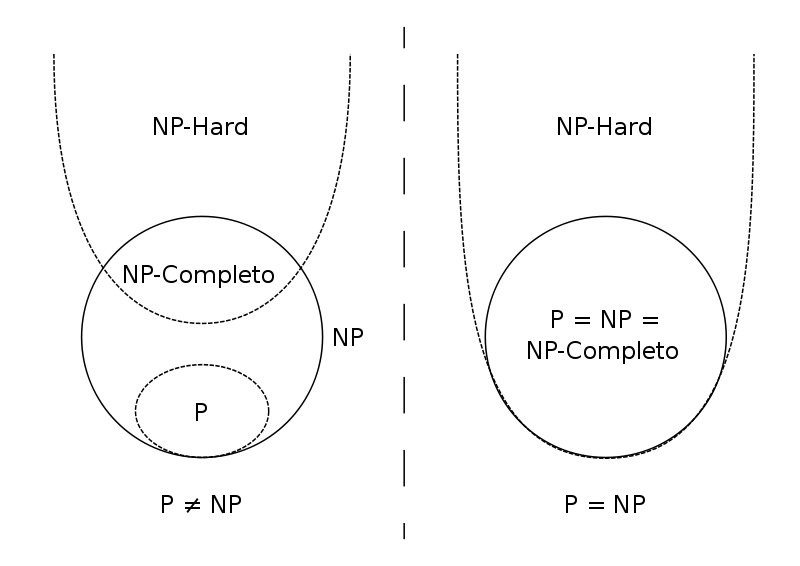
\includegraphics[scale = 0.4]{PNP.png}
		\caption{Diagrama de Euler de las clases de complejidad m\'as frecuentes}
		\label{fig:diagramaEuler}
	\end{figure}
	
	Un ejemplo de problema de optimizaci\'on combinatoria que es \textit{NP-dif\'icil} y que ser\'a el objeto central de estudio de este trabajo es el llamado \textit{problema de empaquetamiento} o \textbf{\textit{Bin Packing Problem}}.
	
	\section{Algoritmos heur\'{\i}sticos y metaheur\'{\i}sticos. Algoritmos evolutivos?}
	
	Como ya se mencion\'o con anterioridad, para muchos problemas de optimizaci\'on combinatoria no se conocen algoritmos que sean capaces de obtener una soluci\'on en tiempo polinomial. Algunos incluso no admiten el uso de algoritmos de aproximaci\'on. En estos casos, nos vemos obligados a usar algoritmos heur\'{\i}sticos.
	\\
	
	Los m\'etodos heur\'{i}sticos son algoritmos que se limitan a proporcionar una "buena" soluci\'on del problema, no necesariamente \'optima, con un coste computacional razonable. Adem\'as, aunque un buen heur\'{\i}stico encuentre muy buenas soluciones para la mayor\'{\i}a de instancias de un problema, no hay garant\'{\i}a de que siempre encuentre una buena soluci\'on para todas las instancias del problema.
	\\
	
	Existen gran cantidad de m\'etodos heur\'{\i}sticos, lo cual hace que sea complicado dar una clasificaci\'on (\textbf{citar Rafael Mart\'{\i}}) de los mismos ya que, por ejemplo, muchos de ellos han sido dise\~{n}ados para resolver un problema concreto. No obstante, podemos dar una clasificaci\'on general donde ubicar a los algoritmos heur\'{\i}sticos m\'as conocidos:
	
	\begin{itemize}
		\item \textbf{M\'etodos de descomposici\'on.} El problema de partida se descompone en subproblemas m\'as sencillos de resolver, sin perder de vista que ambos pertenecen al mismo problema. (\textbf{Ejemplo?})
		\item \textbf{M\'etodos inductivos.} Estos m\'etodos parten de casos m\'as sencillos del problema general, de manera que analizan propiedades o t\'ecnicas que pueden generalizarse al problema completo. (\textbf{Ejemplo?})
		\item \textbf{M\'etodos de reducci\'on.} Consiste en seleccionar propiedades que se verifican de forma general en las soluciones consideradas como buenas e introducirlas como restricciones del problema. La finalidad de estos m\'etodos es restringir el espacio de soluciones para simplificar el problema. El inconveniente que presentan estos m\'etodos, es la posibilidad de dejar fuera del espacio de soluciones nuevo aquellas soluciones \'optimas del problema original. (\textbf{Ejemplo?})
		\item \textbf{M\'etodos constructivos.} Son m\'etodos que construyen paso a paso una soluci\'on del problema. Normalmente son m\'etodos deterministas y suelen estar basados en la mejor elecci\'on en cada iteraci\'on. (\textbf{Ejemplo?} - algoritmos voraces)
		\item \textbf{M\'etodos de b\'usqueda local.} A diferencia de los m\'etodos anteriores, los algoritmos de b\'usqueda o mejora local comienzan con una soluci\'on del problema y la mejoran progresivamente. El algoritmo realiza en cada iteraci\'on un movimiento de una soluci\'on a otra mejor. El m\'etodo finaliza cuando, para una soluci\'on, no existe ninguna otra accesible que la mejore. (\textbf{Ejemplo?} - cualquier algoritmo iterativo?)
	\end{itemize}
	
	Cuando se resuelve un problema por m\'etodos heur\'isticos, como la optimalidad no est\'a garantizada, se debe medir la calidad de los resultados. Para ello existen diversos procedimientros, entre los cuales podr\'iamos destacar los siguientes:
	
	(\textbf{citar https://core.ac.uk/download/pdf/236383515.pdf})
	
	\begin{itemize}
		\item \textbf{Comparaci\'on con la soluci\'on \'optima.} Aunque normalmente se recurre al algoritmo aproximado por no existir un m\'etodo exacto para obtener el \'otimo, o por ser \'este computacionalmente muy costoso, en ocasiones puede que dispongamos de un m\'etodo que proporcione el \'optimo para un conjunto limitado de ejemplos. Este conjunto de ejemplos puede servir para medir la calidad del m\'etodo heur\'istico. Normalmente se mide, para cada uno de los ejemplos, la desviaci\'on porcentual de la soluci\'on heur\'istica frente a la \'optima, calculando posteriormente el promedio de dichas desviaciones.
		\item \textbf{Comparaci\'on con una cota.}  En ocasiones el \'optimo del problema no est\'a disponible ni siquiera para un conjunto limitado de ejemplos. Un m\'etodo alternativo de evaluaci\'on consiste en comparar el valor de la soluci\'on que proporciona el heur\'istico con una cota del problema (inferior si el problema es de minimizar y superior si es de maximizar). La bondad de esta medida depender\'a de la bondad de la cota, es decir, de c\'omo de cercana se encuentre del \'optimo del problema, por lo que de alguna manera, tendremos que tener informaci\'on de lo buena que es dicha cota. En caso contrario, la comparaci\'on propuesta no resulta de utilidad.
		\item \textbf{Comparaci\'on con un m\'etodo exacto truncado.} Para ello elegimos un m\'etodo exacto que resuelva el problema y establecemos un l\'imite de iteraciones o de tiempo m\'aximo conforme a una serie de criterios que nos garanticen que de esta forma obtenemos una buena soluci\'on. Una vez hecho esto, usamos esta soluci\'on para compararla con la que obtenemos seg\'un el heur\'istico. Evidentemente, en este caso suponemos que la resoluci\'on del problema mediante cualquier m\'etodo exacto es inabordable por el coste computacional que requiere.
		\item \textbf{Comparaci\'on con otros heur\'isticos.} Es un m\'etodo usado usalmente en problemas NP-duros para los que se conocen buenos heur\'isticos.
		\item \textbf{An\'alisis del peor caso.} Consiste en considerar los ejemplos que sean m\'as desfavorables para el algoritmo y acotar la m\'axima desviaci\'on respecto del \'optimo del problema. De esta forma, conseguimos acotar el resultado del algoritmo para cualquier ejemplo. Lo malo es que los resultados no suelen ser representativos del comportamiento medio del algoritmo.
	\end{itemize}
	
	Si bien todos estos m\'etodos han contribuido a ampliar nuestro conocimiento para la resoluci\'on de problemas reales, los m\'etodos constructivos y los de b\'usqueda local constituyen la base de los procedimientos metaheur\'isticos.
	\\
	
	Los metahur\'isticos son m\'etodos para dise\~{n}ar y/o mejorar los heur\'isticos en los que estos m\'etodos cl\'asicos no son efectivos a la hora de resolver un problema dif\'icil de optimizaci\'on combinatoria. Son algoritmos h\'ibridos que combinan conceptos de distintos campos como la gen\'etica, la biolog\'ia, la f\'isica, las matem\'aticas, la inteligencia artificial o la neurolog\'ia, por ejemplo. Algunos de los m\'as comunes son los siguientes:
	
	\begin{itemize}
		\item \textbf{Metaheur\'isticos inspiradas en la f\'isica:} Como ya se ha mencionado con anterioridad, el recocido simulado  es un ejemplo de este tipo de algoritmos. Es una t\'ecnica de b\'usqueda inspirada en el proceso de calentamiento y posterior enfriamiento de un metal para obtener estados de baja energ\'ia en un s\'olido. 
		\item \textbf{Metaheur\'isticos inspiradas en la evoluci\'on:} Son m\'etodos que van construyendo una soluci\'on en cada iteraci\'on. Consiste en generar, seleccionar, combinar y reemplazar un conjunto de soluciones en la b\'usqueda de la mejor soluci\'on. Un ejemplo de estos m\'etodos son los algoritmos gen\'eticos. 
		\item \textbf{Metaheur\'isticos inspiradas en la biolog\'ia:} Un ejemplo relativamente reciente de este tipo de algoritmos es la optimizaci\'on basada en colonias de hormigas (ant colony optimization). Se inspira en el comportamiento estructurado que siguen las colonias de hormigas donde los individuos se comunican entre s\'i por medio de las feromonas; la repetici\'on de recorridos por los individuos establece el camino m\'as adecuado entre su nido y su fuente de alimentos. El m\'etodo consiste en simular la comunicaci\'on indirecta que utilizan las hormigas para establecer el camino m\'as corto, guardando la informaci\'on aprendida en una matriz de feromonas.
	\end{itemize}
	
	
	
	
	\chapter{Problema del Bin Packing}
	
	\section{Introducci\'on}
	Existen diversas formulaciones para el problema de Bin Packing, al que nos referiremos de ahora en adelante de manera abreviada como BP o BPP. De forma sencilla, podemos enunciarlo como:
	
	\begin{center}
		Dados \textit{n} objetos de tama\~{n}o $w_{1},..., w_{n}$, queremos encontrar el menor n\'umero de cubos de tama\~{n}o \textit{c} en donde se coloquen todos los objetos.
	\end{center}
	
	A los objetos $w_{i}$ anteriores se les denomina habitualmente pesos. Son m\'ultiples las aplicaciones que tienen los problemas de tipo BP, adem\'as que podemos considerar variantes multidimensionales: desde el llenado de contenedores y/o camiones con restricciones de volumen y peso a la creaci\'on de copias de seguridad de archivos o una asignaci\'on eficiente de la memoria de un ordenador. 
	\\
	
	Como vemos, es un problema d\'ificil de resolver debido a que su complejidad crece exponencialmente con el n\'umero de objetos a almacenar y variables a considerar, como por ejemplo si dichos objetos fueran tridimensionales y tuvi\'eramos que considerar su volumen y su peso a la hora de imponer las restricciones del problema. Resulta aqu\'i visible la dificultad que presentan los problemas de optimizaci\'on combinatoria y la necesidad de desarrollar algoritmos suficientemente buenos que puedan resolverlos en tiempos aceptables.
	
	\begin{observacion}
		Cuando el n\'umero de cubos se limita a uno y cada objeto se caracteriza por su peso y su volument, el problema de maximizar el peso de los objetos que pueden caber en el contenedor se conoce como el  ya mencionado problema de la mochila.
	\end{observacion}
	
	El BPP tambi\'en puede considerarse como un caso especial del \textit{cutting stock problem}, cuyo origen est\'a asociado a la industria maderera: (citar wiki)
	\\
	
	Consideremos una lista de \textit{m} \'ordenes para las cuales se requiere $q_{j}$, $j = 1,...,m$ piezas para cada una. Posteriormente, se construye una lista de todas las combinaciones posibles de los recortes (frecuentemente llamados \textit{patrones}), asociando a cada uno de ellos una variable entera positiva $x_{i}$ que representa cuantas veces ser\'a utilizado cada patr\'on. Entonces, el problema de programaci\'on lineal entera se modeliza matem\'aticamente como
	\newpage
	
	$$ min \sum_{i=1}^{n}c_{i}x_{i} $$
	$$ s.a\, \sum_{i=1}^{n}a_{ij}x_{i},\, \forall j=1,...,m $$
	$$ x_{i}\in \mathbb{Z^{+}},\, \forall i=1,...,n $$
	\\
	donde $a_{ij}$ es el n\'umero de veces que en la orden \textit{j} aparece el patr\'on \textit{i} y $c_{i}$ es el costo (a menudo llamado \textit{residuo}) del patr\'on \textit{i}. Cuando $c_{i} = 1$ la funci\'on objetivo minimiza el n\'umero de elementos utilizados y, si larestricci\'on de los elementos a producir se sustituye por la igualdad, obtenemos el BPP (\textbf{esta parte no la entiendo}). As\'i, procedemos a continuaci\'on a formular matem\'aticamente el problema BP.
	\\
	
	Sea \textit{n} objetos (items) y \textit{n} cubos (bins), donde
	
	$$w_{j} = \mbox{peso del item \textit{j}},$$
	$$c = \mbox{capacidad de cada cubo},$$
	\\
	entonces 
	
	$$ min \sum_{i=1}^{n}y_{i} $$
	$$ s.a\, \sum_{j=1}^{n}w_{j}x_{ij} \leq cy_{i},\, \forall i=1,...,n $$
	$$ \sum_{i=1}^{n}x_{ij} = 1,\, \forall j=1,...,n $$
	\\
	donde
	
	\[y_{i} = \left\{\begin{array}{ll}
		1 \hspace{0.5cm} \text{si se usa el bin \textit{i}}\\
		0 \hspace{0.5cm} \text{en otro caso}
	\end{array}\right.\]
	\\
	\[x_{ij} = \left\{\begin{array}{ll}
		1 \hspace{0.5cm} \text{si el item \textit{j} se asigna al bin \textit{i}}\\
		0 \hspace{0.5cm} \text{en otro caso}
	\end{array}\right.\]
	\\
	Supondremos, adem\'as, que los pesos $w_{j}$ son enteros positivos. Por lo tanto, sin p\'erdida de generalidad, podemos suponer que
	
	$$ c \mbox{es un entero positivo,} $$
	$$ w_{j} \leq c,\, \forall j = 1,...,n. $$
	\\
	Si alg\'un item no verifica la \'ultima suposici\'on, entonces el problema es trivialmente imposible.
	\\
	
	En lo que sige, propondremos una serie de algoritmos con los que aproximar las soluciones de distintas instancias del problema BP, a la par que analizaremos c\'omo de buenos son y a qu\'e coste. Para ello, el primer tipo de m\'etodos que analizaremos ser\'an los algoritmos voraces (\textit{greedy alhorithm}).
	
	\section{Algoritmos voraces}
	Por algoritmos voraces se entienden aquellos algoritmos que siguen un esquema de resoluci\'on llamado m\'etodo voraz. Dicho esquema forma parte de una familia de algoritmos m\'as amplia denominada \textit{algoritmos de b\'usqueda local}, de la que tambi\'en forman parte, por ejemplo, el m\'etodo del gradiente, los algoritmos gen\'eticos o los algoritmos de cristalizaci\'on simulada. Los algoritmos que siguen este m\'etodo son, en general, los que menos dificultades plantean a la hora de implementar y comprobar su funcionamiento, y suelen aplicarse en problemas de optimizaci\'on.
	\\
	
	Frecuentemente, los algoritmos de tipo greedy y los problemas que pueden resolver, se caracterizan por la mayor\'ia de las siguientes caracter\'isticas (\textbf{citar Brassard}):
	
	\begin{itemize}
		\item Tenemos que resolver un problema de optimizaci\'on y, para construir su soluci\'on, tenemos un conjunto de candidatos: en el caso que nos ata\~{n}e, esos candidatos resultan ser los objetos que queremos introducir en los cubos.
		\item A medida que el algoritmo avanza, tenemos otros dos conjuntos. Por un lado, tenemos el conjunto formado por los candidatos que ya han sido considerados y elegidos, mientras que por otro tenemos el conjunto con los candidatos que han sido considerados y rechazados.
		\item Hay una funci\'on que verifica si un conjunto particular de candidatos es una soluci\'on del problema, independientemente de si dicha soluci\'on es la \'optima.
		\item Hay otra funci\'on que verifica si un conjunto de candidatos es factible, es decir, si es posible o no completar el conjunto a\~{n}adiendo m\'as candidatos hasta obtener al menos una soluci\'on del problema. De nuevo, esta funci\'on tampoco tiene en cuenta la optimalidad de dicha soluci\'on.
		\item Una funci\'on m\'as, llamada funci\'on de selecci\'on, que indica en cada momento cual de los candidatos restantes, que no han sido elegidos ni rechazados, es el que podr\'ia ser el mejor.
		\item Finalmente, una funci\'on objetivo que nos proporciona el valor de la soluci\'on que hemos encontrado. En nuestro problema de BP, dicha funci\'on
		es el n\'umero de bins a minimizar y, a diferencia de las tres funciones
		anteriores, la funci\'on objetivo no aparece expl\'icitamente en el algoritmo.
	\end{itemize}
	
	Un algoritmo voraz avanza paso a paso. Esto quiere decir que, inicialmente,
	el conjunto de los candidatos elegidos est\'a vac\'io. Luego, en cada paso, la funci\'on de selecci\'on elige al mejor candidato restante sin parar a considerar si lo introducimos o no en el conjunto anterior. Si el conjunto ampliado de candidatos elegidos ya no es factible, rechazamos el candidato que estamos considerando actualmente. En este caso, el candidato con el que hemos probado y que ha sido rechazado no se vuelve a considerar de nuevo. En cambio, si el conjunto ampliado es factible, a\~{n}adimos el candidato al conjunto de los candidatos elegidos. Cada vez que ampliamos dicho conjunto, verificamos si en ese momento este conjunto es una soluci\'on del problema. De esta forma, un algoritmo voraz se ver\'ia de la siguiente forma:
	\\
	
	\noindent\fbox{
		\begin{minipage}{0.5\textwidth}
			\begin{algorithmic}
				
				\State{funci\'on greedy (C: set): set}
				\State{//C es el conjunto de los candidatos}
				\State{//Construimos la soluci\'on en el conjunto S}
				\State{S = $\emptyset$}\
				\While{(C $\neq \emptyset$ \textbf{y no} solucion(S))}
				\State{$x \longleftarrow seleccionar(C)$}
				\State{$C \longleftarrow C-\{x\}$}
				\If{($factible(S\cup \{x\})$)}
				\State{$S \longleftarrow S\cup \{x\}$}
				\EndIf
				\EndWhile
				\If{(solucion(S))}
				\State{\textbf{return} S}
				\Else
				\State{\textbf{return} "No hay soluci\'on"}
				\EndIf
				
			\end{algorithmic}
		\end{minipage}
	}
	\\\\
	
	A continuaci\'on, pasamos a presentar los algoritmos voraces con los que ofreceremos distintas soluciones del problema del BP. Daremos una breve explicaci\'on del funcionamiento de los algoritmos, sus pseudoc\'odigos y analizaremos sus complejidades. 
	
	
	\subsection{Primeras aproximaciones}
	\subsubsection{Next Fit}
	Este algoritmo es el m\'as sencillo de implementar y con el que obtener una r\'apida soluci\'on del problema, aunque no muy buena. Funciona de la siguiente manera: comenzamos con una soluci\'on en la que no tenemos ning\'un cubo. A continuaci\'on, seleccionamos el primer objeto de la lista de objetos que queremos introducir en los cubos y lo introducimos en un nuevo cubo dado que es el primer elemento seleccionado. Para los siguientes objetos, el algoritmo comprueba si podemos introducir el elemento seleccionado en el \'ultimo cubo creado. Si se puede, lo introducimos. En otro caso, creamos un cubo nuevo y lo introducimos.
	\\
	
	Vemos que, aunque es un algoritmo que nos permite obtener una soluci\'on de manera sencilla y r\'apida (puesto que no hay muchas comprobaciones que realizar), no resulta muy eficiente como veremos. As\'i, el pseudoc\'odigo del algoritmo ser\'ia el siguiente:
	
	\noindent\fbox{
		\begin{minipage}{\textwidth}
			\begin{algorithmic}
				
				\State{nextFit (capacity: Int, items: Array[Int]): Array[Bin]}
				\State{//capacity es la capacidad de los cubos}
				\State{//items es un array que almacena los elementos que introduciremos en los cubos}
				\State{//El array solution almacenar\'a los cubos y current ser\'a el \'ultimo cubo creado}
				\State{solution = $\emptyset$}\
				\State{current = new Bin(capacity)}\
				\For{(item $\leftarrow$ items)}
				\If{(item cabe en current)}
				\State{A\~{n}adimos el item a current}
				\Else
				\State{A\~{n}adimo current a soltion}
				\State{current = new Bin(capacity)}
				\State{A\~{n}adimos el item a current}
				\EndIf
				\EndFor
				\State{A\~{n}adimos el \'ultimo cubo creado a solution}
				\State{\textbf{return} solution}
				
			\end{algorithmic}
		\end{minipage}
	}
	\\\\
	
	Observemos que, dada una lista de \textit{n} pesos, el algoritmo hace una \'unica comprobaci\'on por cada iteraci\'on. Por lo tanto, tenemos que la complejidad del algoritmo es \textit{O(n)}, con lo que la velocidad de resoluci\'on del problema se incrementa de forma lineal conforme lo hace el n\'umero de elementos que tenemos que introducir en los cubos. As\'i pues, como primera aproximaci\'on, ser\'ia un algoritmo \'util, r\'apido y f\'acil de resolver para instancias peque\~{n}as del problema en las que no estamos interesados en obtener el \'optimo.
	\\
	
	\textbf{QUEDA POR ANALIZAR SU APPROXIMATION RATIO}
	
	\subsubsection{First Fit}
	Podr\'iamos considerar a este algoritmo como un primer intento de mejorar el m\'etodo anterior ya que, aunque no reconsideremos las decisiones tomadas (es decir, si alguno de los items introducidos en los cubos existentes deber\'ia introducirse en otro cubo), que es la idea b\'asica de los algortimos voraces, s\'i que vamos llenando "mejor" los cubos que se van creando en las iteraciones del algoritmo. Adem\'as, posteriormente este ser\'a uno de los algortimos que usaremos como base para implmententar mejores t\'ecnicas de resoluci\'on del problema del BP.
	\\
	
	El algoritmo es el siguiente: empezamos igual que en el caso anterior; partimos de una soluci\'on que no tiene ningu\'un cubo. Seleccionamos el primer elemento de nuestra lista de objetos a introducir en los cubos y creamos un primer cubo donde a\~{n}adimos el elemento. Para los siguientes elementos, recorremos nuestra soluci\'on de cubos y a\~{n}adimos el elemento en el primer cubo que encontremos donde quepa el objeto. Si no hay ning\'un cubo en el que quepa el elemento seleccionado, creamos un nuevo cubo y lo introducimos.
	\\
	
	De esta forma, el pseudoc\'odigo del algoritmo ser\'ia el siguiente:
	\\
	
	\noindent\fbox{
		\begin{minipage}{\textwidth}
			\begin{algorithmic}
				
				\State{firstFit (capacity: Int, items: Array[Int]): Array[Bin]}
				\State{//capacity es la capacidad de los cubos}
				\State{//items es un array que almacena los elementos que introduciremos en los cubos}
				\State{//El array solution almacenar\'a los cubos y current ser\'a el \'ultimo cubo creado}
				\State{//Inicializamos el algoritmo con el array de soluciones teniendo un cubo vac\'io}
				\State{current = new Bin(capacity)}\
				\State{A\~{n}adimos el cubo vac\'io a solution}\
				\For{(item $\leftarrow$ items)}
				\State{i = 0}
				\While{(item \textbf{no} est\'e a\~{n}adido \textbf{y} i $\leq$ tama\~{n}o de solution)}
				\If{(El item cabe en el cubo i-\'esimo)}
				\State{A\~{n}adimos el item en el cubo i-\'esimo}
				\Else
				\State{i = i + 1}
				\EndIf
				\EndWhile
				\If{(El item no se ha a\~{n}adido a ning\'un cubo)}
				\State{current = new Bin(capacity)}
				\State{A\~{n}adimos el item a current}
				\State{A\~{n}adimos el cubo current a solution}
				\EndIf
				\EndFor
				\State{\textbf{return} solution}
				
			\end{algorithmic}
		\end{minipage}
	}
	\\\\
	
	Como mencionamos anteriormente, este algoritmo conseguimos mejorar la soluci\'on obtenida seg\'un el m\'etodo Next Fit, pero esto implica que la complejidad algor\'itmica se incrementa. Dado una lista de \textit{n} elementos, el bucle for itera sobre cada uno de ellos, por lo que la complejidad introducida a priori por el bucle es \textit{O(n)}. Pero, a su vez, en cada iteraci\'on el bucle while recorre en el peor de los casos toda la lista de cubos, con lo que su complejidad es tambi\'en \textit{O(n)}. Por lo tanto, la complejidad del algoritmo resulta ser \textit{O(n)}.
	\\
	
	\textbf{QUEDA POR ANALIZAR SU APPROXIMATION RATIO}
	
	\subsubsection{Best Fit}
	Este es el primero de los algoritmos que intenta ofrecernos una mejora "considerable" a la hora de llenar los cubos ya que no solo intenta ir llenando todos los cubos en cada iteraci\'on, sino que los llena de la mejor forma posible, entendiendo esa forma mejor como aquella en la que el elemento seleccionado llena mejor en el cubo. Al igual que el first fit y los m\'etodos posteriores, las mejoras que conseguimos en busca de la soluci\'on \'optima o una aproximada, aparecen a costa de incrementar la complejidad del algoritmo.
	\\
	
	De esta forma, el algoritmo best fit es: seleccionamos el primer objeto de nuestra lista, creamos un nuevo cubo con la capacidad dada en el problema e introducimos el objeto. Para los siguientes elementos buscamos el cubo cuya capacidad restante sea menor y que, adem\'as, quepa el elemento. Si encontramos un cubo que cumpla esta condici\'on introducimos el objeto. En otro caso, creamos un cubo nuevo y lo introducimos.
	\\
	
	Obs\'ervese que aquel cubo donde se verifiquen las condiciones dadas para introducir un nuevo elemento no tiene por qu\'e ser \'unico. Por lo tanto, a la hora de implementar el algoritmo iremos insertando los cubos en nuestra soluci\'on de manera ordenada, con lo que cuando vayamos a seleccionar en qu\'e cubo introducimos un nuevo elemento cuando haya m\'as de una elecci\'on posible, lo haremos eligiendo el primer cubo que encontremos. As\'i, el pseudoc\'odigo del algoritmo queda como sigue: 
	\\
	
	\noindent\fbox{
		\begin{minipage}{\textwidth}
			\begin{algorithmic}
				
				\State{bestFit (capacity: Int, items: Array[Int]): Array[Bin]}
				\State{//capacity es la capacidad de los cubos}
				\State{//items es un array que almacena los elementos que introduciremos en los cubos}
				\State{//El array solution almacenar\'a los cubos y current ser\'a el \'ultimo cubo creado}
				\State{//Inicializamos el algoritmo con el array de soluciones sin ning\'un cubo}
				\State{//targetBin es la posici\'on en solution del cubo con la menor capacidad restante que es mayor o igual que el peso del item seleccionado}
				\State{//smallerThanTarget es un m\'etodo de b\'usqueda binaria con el que, dado un array y un elemento, encuentra la posici\'on del menor elemento del array que es mayor o igual que el elemento dado}
				\State{solution = $\emptyset$}\
				\For{(item $\leftarrow$ items)}
				\State{targetBin = 1 + smallerThanTarget(item, solution)}
				\If{(targetBin $>$ 0 \textbf{y} targetBin $\leq$ longitud de solution - 1)}
				\State{A\~{n}adimo el item en el cubo que se encuentra en la posicion targetBin}
				\State{Reordenamos el array solution de menor a mayor capacidad restante}
				\Else
				\State{current = new Bin(capacity)}
				\State{A\~{n}adimo el item en el cubo current}
				\State{A\~{n}adimo el cubo current en solution}
				\State{Reordenamos el array solution de menor a mayor capacidad restante}
				\EndIf
				\EndFor
				\State{\textbf{return} solution}
				
			\end{algorithmic}
		\end{minipage}
	}
	\\\\
	
	Como ya veremos en el cap\'itulo dedicado a explicar la implementaci\'on de los m\'etodos aqu\'i descritos, lo primero que debemos tener en cuenta para analizar la complejidad de este algoritmo es que, en cada iteraci\'on, para localizar el cubo donde el objeto seleccionado quede m\'as ajustado realizamos una b\'usqueda binaria con el m\'etodo \textit{smallerThanTarget}, que es \textit{O(log n)}. Por otro lado, tras insertar el elemento, la capacidad del cubo disminuir\'a, con lo que tendremos que desplazarlo a la izquierda (ya que en nuestra implementaci\'on ordenaremos los cubos de menor a mayor capacidad restante) para seguir manteniendo los cubos en orden. En el peor de los casos, este desplazamiento ser\'a \textit{O(n)} si, por ejemplo, tenemos que desplazar un cubo que est\'a en el extremo derecho al extremo izquierdo.
	\\
	
	Por lo tanto, cada iteraci\'on en la que insertamos un nuevo elemento ser\'a \textit{O(log n)} + \textit{O(n)} = \textit{O(n)}. De esta forma, como tenemos que insertar \textit{n} elementos, el coste total del algoritmo ser\'a $n \cdot O(n) = O(n^{2})$.
	
	\subsubsection{Worst Fit}
	El m\'etodo Worst Fit es una variante del algoritmo Best Fit. Mientras que en el m\'etodo Best Fit vamos introduciendo los pesos en aquellos cubos que quepan y que tengan la menor capacidad restante posible, en el Worst Fit los introducimos en los cubos que quepan y que, adem\'as, tengan la mayor capacidad restante de entre todos ellos. Tambi\'en, al igual que en el m\'etodo Best Fit, a la hora de implementar el algoritmo tenemos la soluci\'on con los cubos ordenados de menor a mayor capacidad restante. As\'i, como tenemos que elegir aquel cubo con la mayor capacidad restante, lo \'unico que tendremos que comprobar en cada iteraci\'on del algoritmo es que el peso seleccionado quepa en el \'ultimo cubo de la soluci\'on.
	\\
	
	As\'i, el algoritmo quedar\'ia: inicializamos el algoritmo igual que en Best Fit, partiendo de una soluci\'on que tiene un cubo en el cual introducimos el primer peso. A continuaci\'on, para cada elemento buscamos aquel cubo con la mayor capacidad restante y en el que quepa el elemento. Si lo encontramos, introducimos el peso. En otro caso creamos un cubo nuevo, introducimos el elemento y a\~{n}adimos el cubo a la soluci\'on. Por lo tanto, el pseudoc\'odigo del algoritmo quedar\'ia como:
	\\
	
	\noindent\fbox{
		\begin{minipage}{\textwidth}
			\begin{algorithmic}
				
				\State{worstFit (capacity: Int, items: Array[Int]): Array[Bin]}
				\State{//capacity es la capacidad de los cubos}
				\State{//items es un array que almacena los elementos que introduciremos en los cubos}
				\State{//El array solution almacenar\'a los cubos y current ser\'a el \'ultimo cubo creado}    
				\State{//targetBin es la posici\'on en solution del cubo con la menor capacidad restante que es mayor o igual que el peso del item seleccionado}
				\State{//smallerThanTarget es un m\'etodo con el que, dado un array y un elemento, encuentra la posici\'on del menor elemento del array que es mayor o igual que el elemento dado}
				\State{//Inicializamos el algoritmo con el array de soluciones sin ning\'un cubo}
				\State{solution = $\emptyset$}\
				\For{(item $\leftarrow$ items)}
				\State{targetBin = smallerThanTarget(item, solution)}
				\If{(targetBin es menor que la longitud de solution)}
				\State{//Esto equivale a comprobar que item cabe en el \'ultimo cubo}
				\State{A\~{n}adimo el item en el cubo que se encuentra en la \'ultima posici\'on}
				\State{Reordenamos el array solution de menor a mayor capacidad restante}
				\Else
				\State{current = new Bin(capacity)}
				\State{A\~{n}adimo el item en el cubo current}
				\State{A\~{n}adimo el cubo current en solution}
				\State{Reordenamos el array solution de menor a mayor capacidad restante}
				\EndIf
				\EndFor
				\State{\textbf{return} solution}
				
			\end{algorithmic}
		\end{minipage}
	}
	\\\\
	
	\textbf{QUEDA POR ANALIZAR LA COMPLEJIDAD DEL ALGORITMO}
	\\
	
	De aqu\'i en adelante los m\'etodos que emplearemos para buscar mejores soluciones para el problema del BP utilizar\'an de base las t\'ecnicas anteriores. No obstante, antes de llegar a ellos podemos mencionar una serie de variaciones de los algoritmos anteriores que, en funci\'on de la instancia del problema que estemos considerando, pueden ofrecer mejores soluciones que los algoritmos que hemos visto hasta ahora.
	\\
	
	
	
	
	
	
	
	
	
	\subsection{Subsecci\'{o}n}
	Una secci\'{o}n dentro de una secci\'{o}n se denomina subsecci\'{o}n.
	\subsubsection{Subsubsecci\'{o}n}
	Esto es una secci\'{o}n dentro de una subsecci\'{o}n, o sea, una subsubsecci\'{o}n.
	Esto es un ejemplo de cita \cite{Zfinitegrading}
	
	\addcontentsline{toc}{chapter}{Bibliograf\'{\i}a}
	\bibliographystyle{plain}
	\bibliography{ref}% Crear archivo bib con referencias en bibtex
	
	
	
	
\end{document}
